\minitoc

\vfill

In Chapters~\ref{chap::semantic_evaluation} and~\ref{chap::learned_evaluation}, we proposed a semantic quality evaluation of building \gls{acr::3d} models employing a learning formulation.
Herein, we aim at puting our pipeline to the test using the obtained dataset.
First, in Section~\ref{sec::experiments::datasets}, we delineate how the building models were obtained.
Second and last, Section~\ref{sec::experiments::evaluation} experimentally provides a first outlook of the capacity of our approach to detect errors affecting building \gls{acr::3d} models.

\clearpage

\section{\textsc{Datasets}}
    \label{sec::experiments::datasets}
    
    \subsection{\textsc{Data preprocesing}}
        \label{subsec::experiments::datasets::preprocessing}

    \subsection{\textsc{Urban scenes and modeling techniques}}
        \label{subsec::experiments::datasets::scenes}
        \gls{acr::3d} models from three different cities of France are selected in order to assess the performance of our framework: \textbf{Elancourt}, \textbf{Nantes}, and the XIII\textsuperscript{th} district of Paris (\textbf{Paris-13}) (\textit{cf.} Figure~\ref{fig::france_map}).
        Figure~\ref{fig::elancourt_ortho} depicts the small city of \textbf{Elancourt} which contains diverse of building types: residential areas with gable and hip roof buildings and large industrial flat roof building based districts (\textit{cf.} Subfigure~\ref{subfig::elancourt_samples}).
        \textbf{Nantes}, as shown in Figure~\ref{fig::nantes_ortho}, represents a denser urban setting but with a lower building diversity (\textit{cf.} Subfigure~\ref{subfig::nantes_samples}).
        In Figure~\ref{fig::paris-13_ortho}, one can see how \textbf{Paris-13} consists of mostly flat roof high towers which coexist with Haussmann style buildings that typically exhibit highly fragmented roofs (\textit{cf.} Subfigure~\ref{subfig::paris-13_samples}).
        The \textbf{Elancourt} (\textit{resp.} \textbf{Nantes} and \textbf{Paris-13}) scene contains 2,009 (\textit{resp.} 748 and 478) annotated building models.
        The \gls{acr::dsm} as well as the orthorectified image resolution is \SI{0.06}{\m} for the first area while it is \SI{0.1}{\m} for the other ones.

        \begin{figure}[htpb]
            \ffigbox[\textwidth]{
                \includegraphics[width=.75\textwidth]{images/datasets/france_map}
            }{
                \label{fig::france_map}
                \caption{
                    Map of France showing the studied urban scenes.
                    Each square corresponds to a city:
                    \textcolor[rgb]{.84,.1,.11}{\(\blacksquare\)} \textbf{Paris-13}, \textcolor[rgb]{1,.79,.5}{\(\blacksquare\)} \textbf{Elancourt}, \textcolor[rgb]{.17,.51,.73}{\(\blacksquare\)} \textbf{Nantes}.
                }
            }
        \end{figure}

        \begin{figure}[htpb]
            \ffigbox[\FBwidth]{
                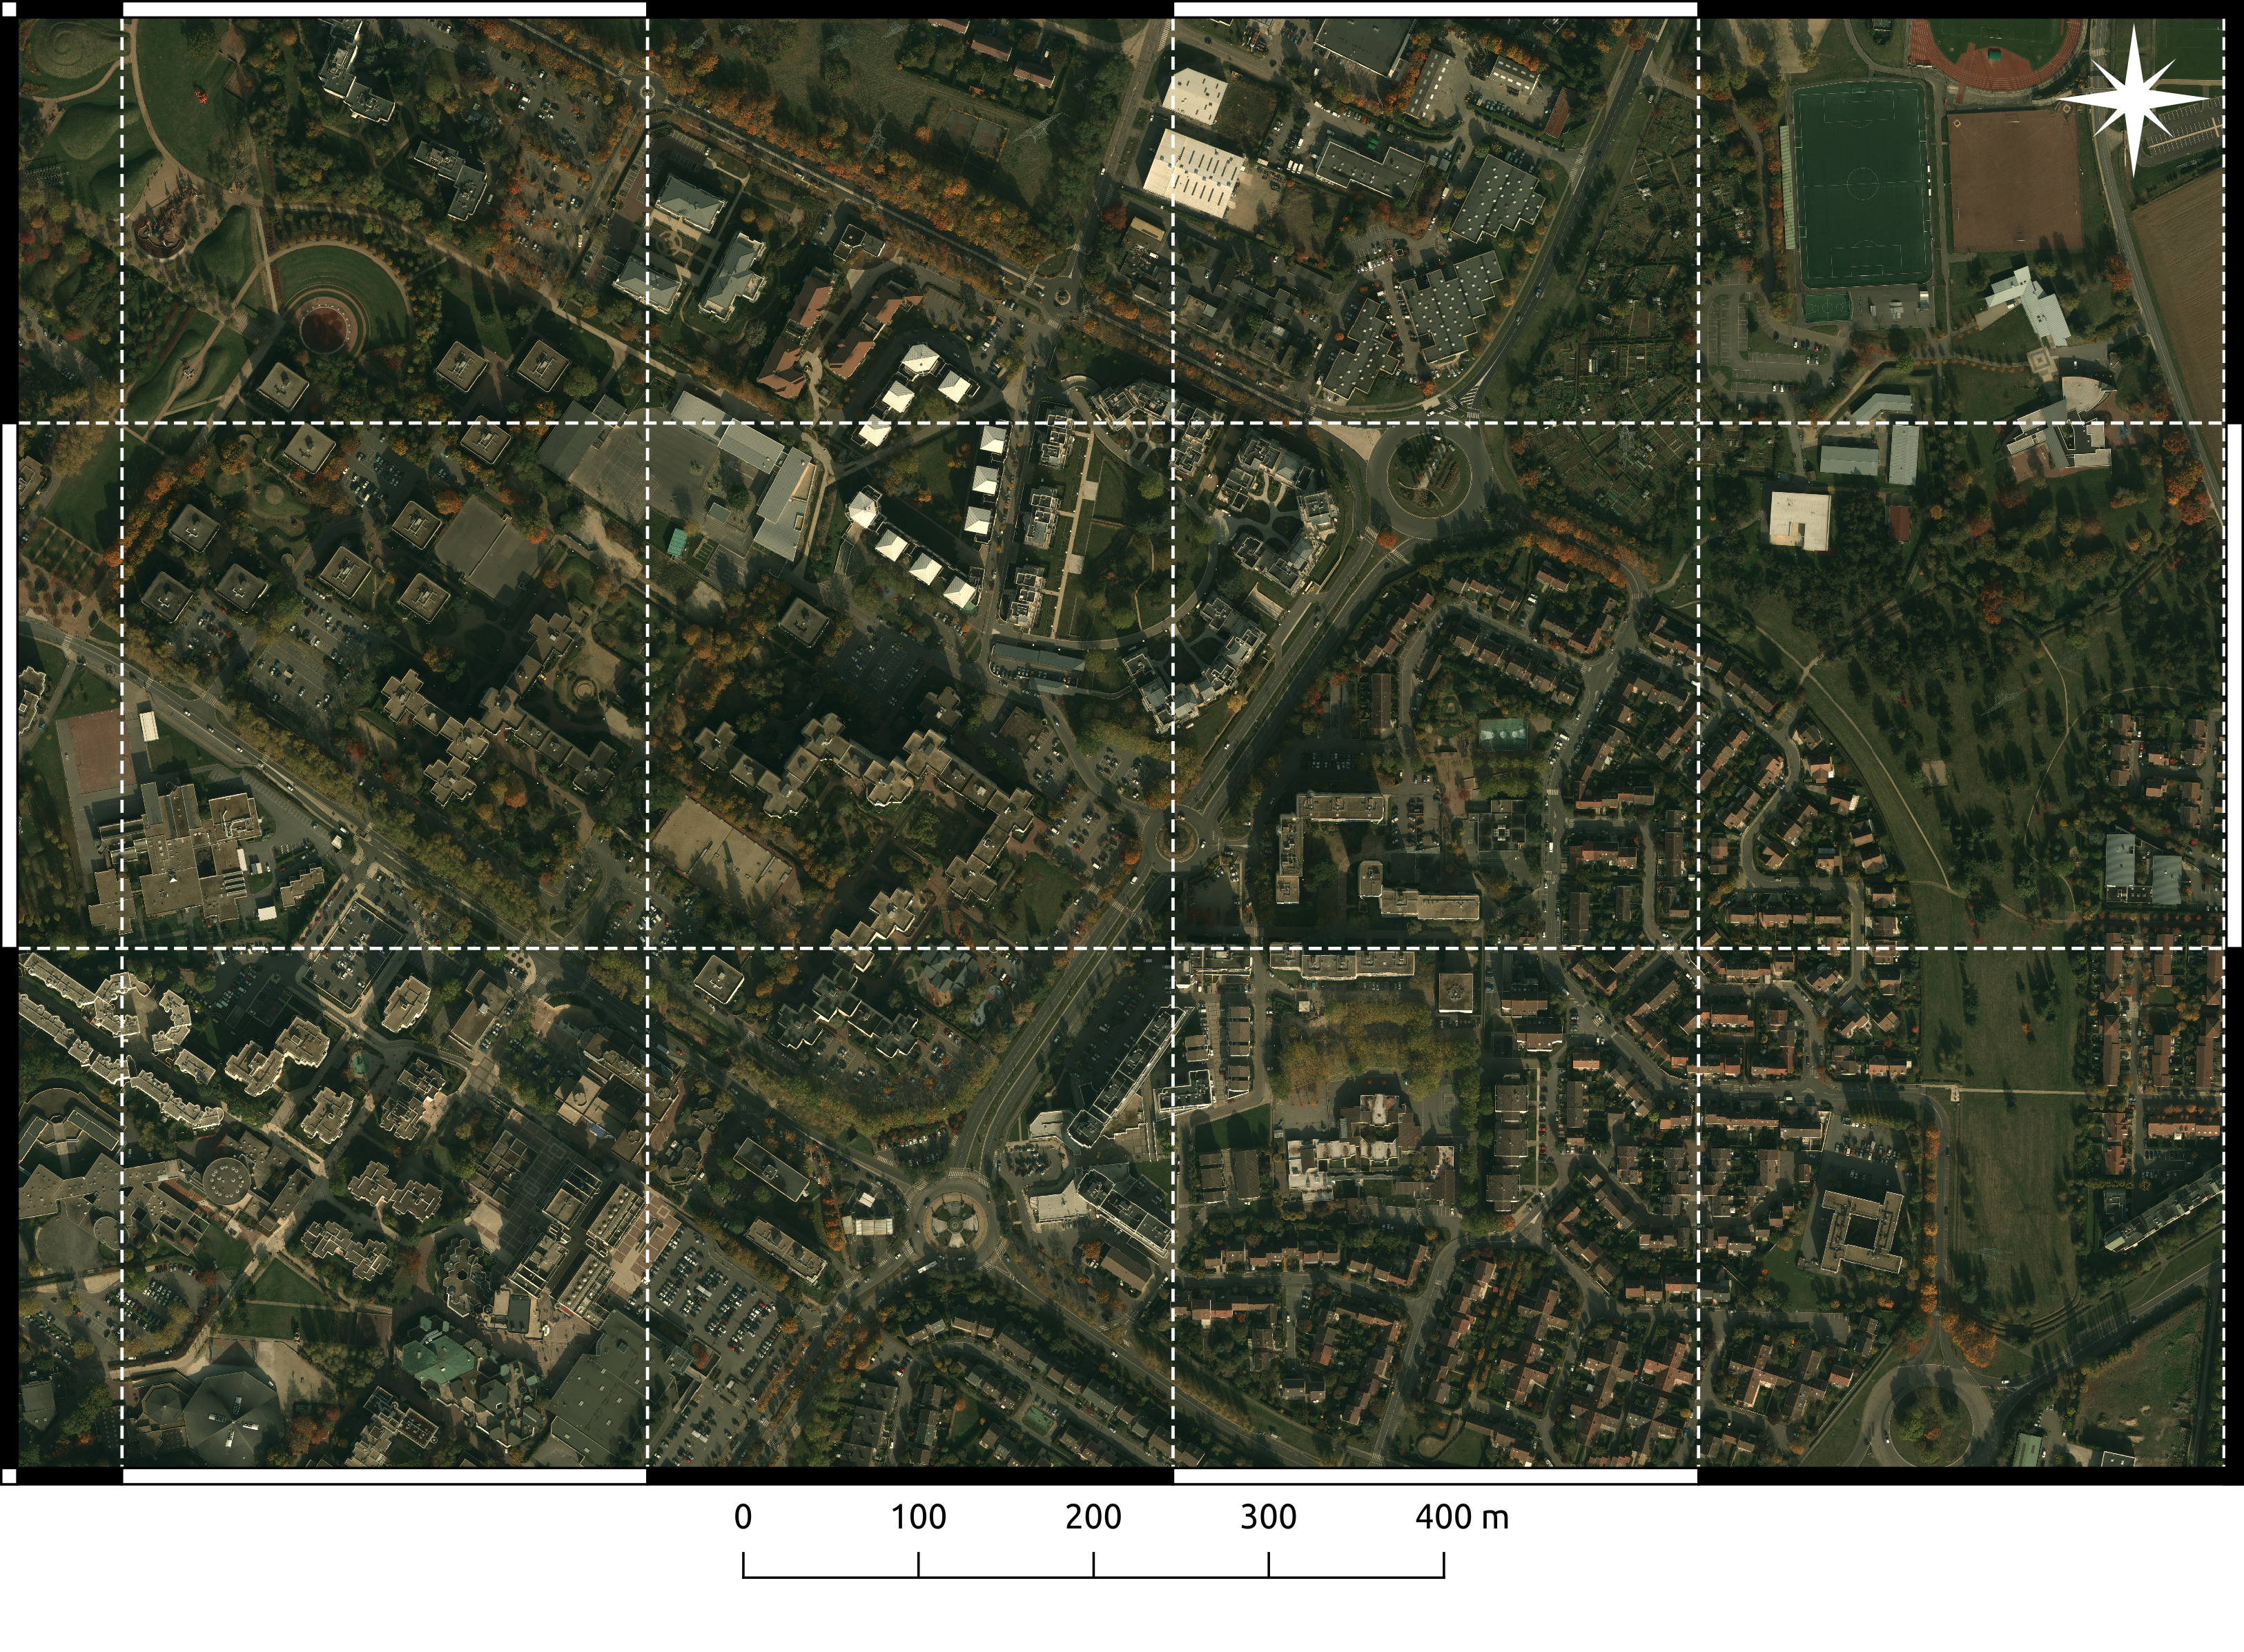
\includegraphics[width=\textwidth]{images/datasets/elancourt_global}
            }{
                \label{fig::elancourt_ortho}
                \caption{
                    Orthoimage showing the diversity of buildings in Elancourt.
                }
            }
        \end{figure}

        \begin{figure}[htpb]
            \ffigbox[\FBwidth]{
                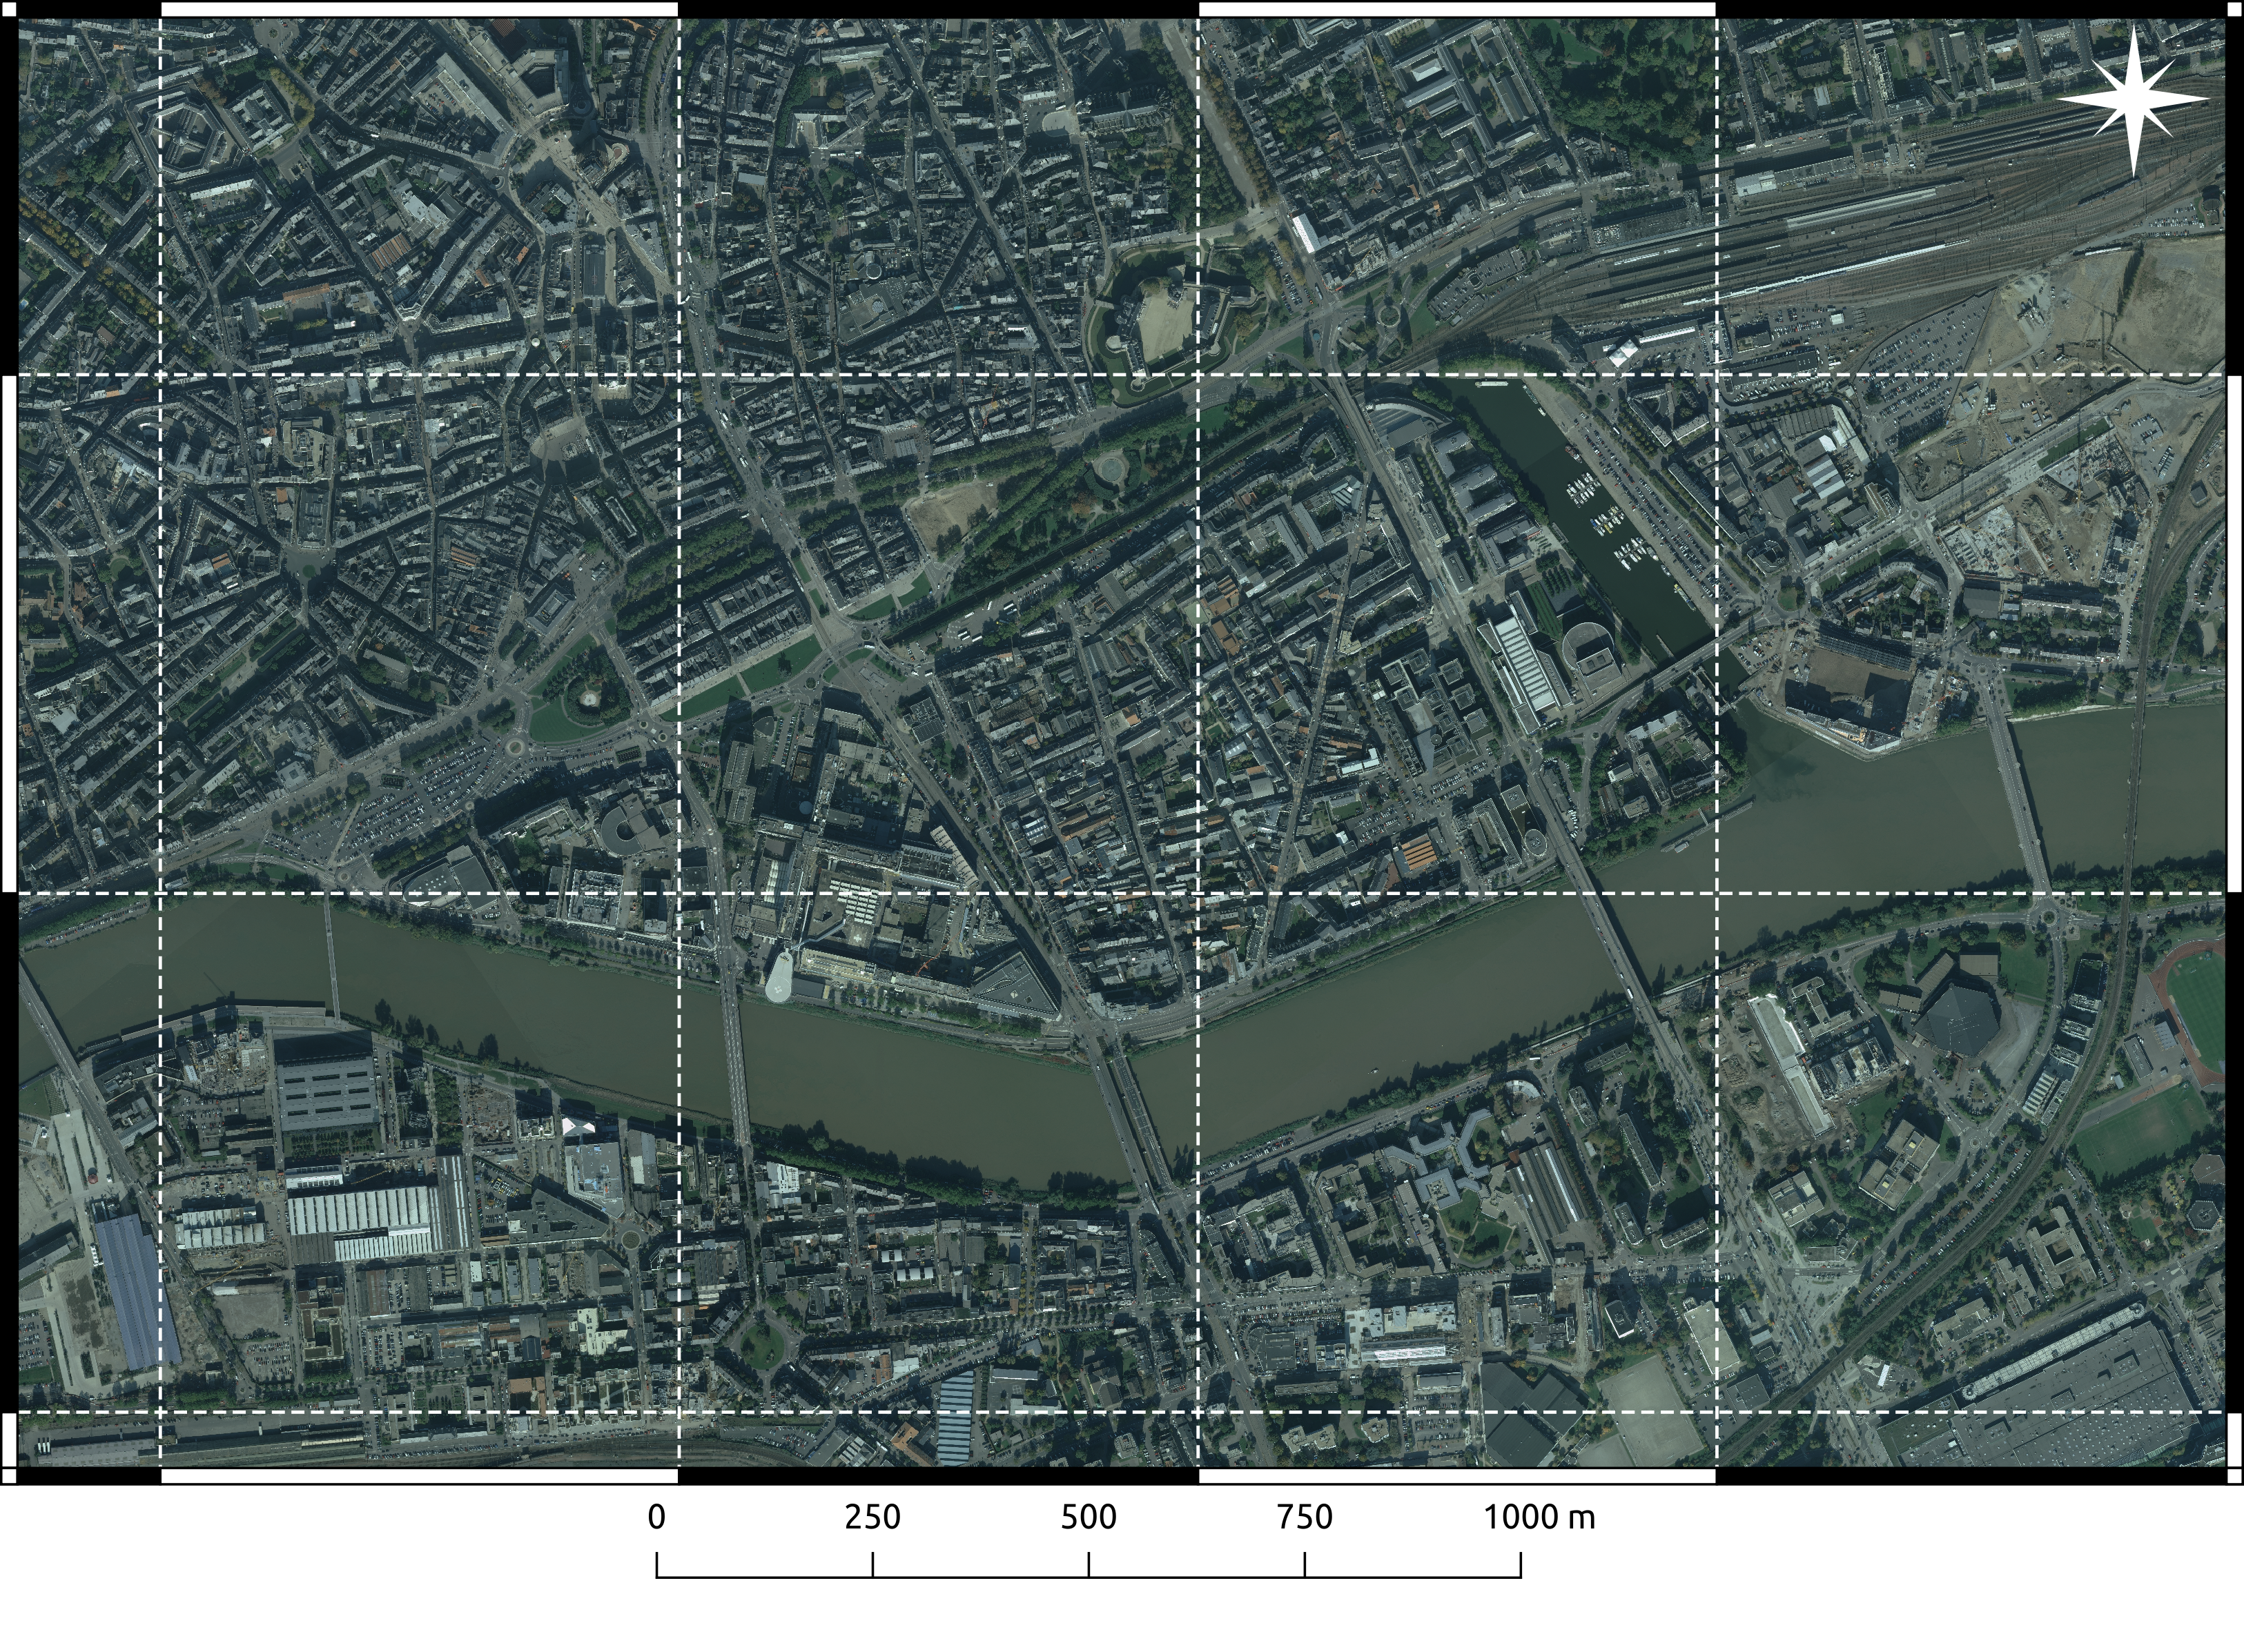
\includegraphics[width=\textwidth]{images/datasets/nantes_global}
            }{
                \label{fig::nantes_ortho}
                \caption{
                    Orthoimage depicting the dense city center of Nantes.
                }
            }
        \end{figure}

        \begin{figure}[htpb]
            \ffigbox[\FBwidth]{
                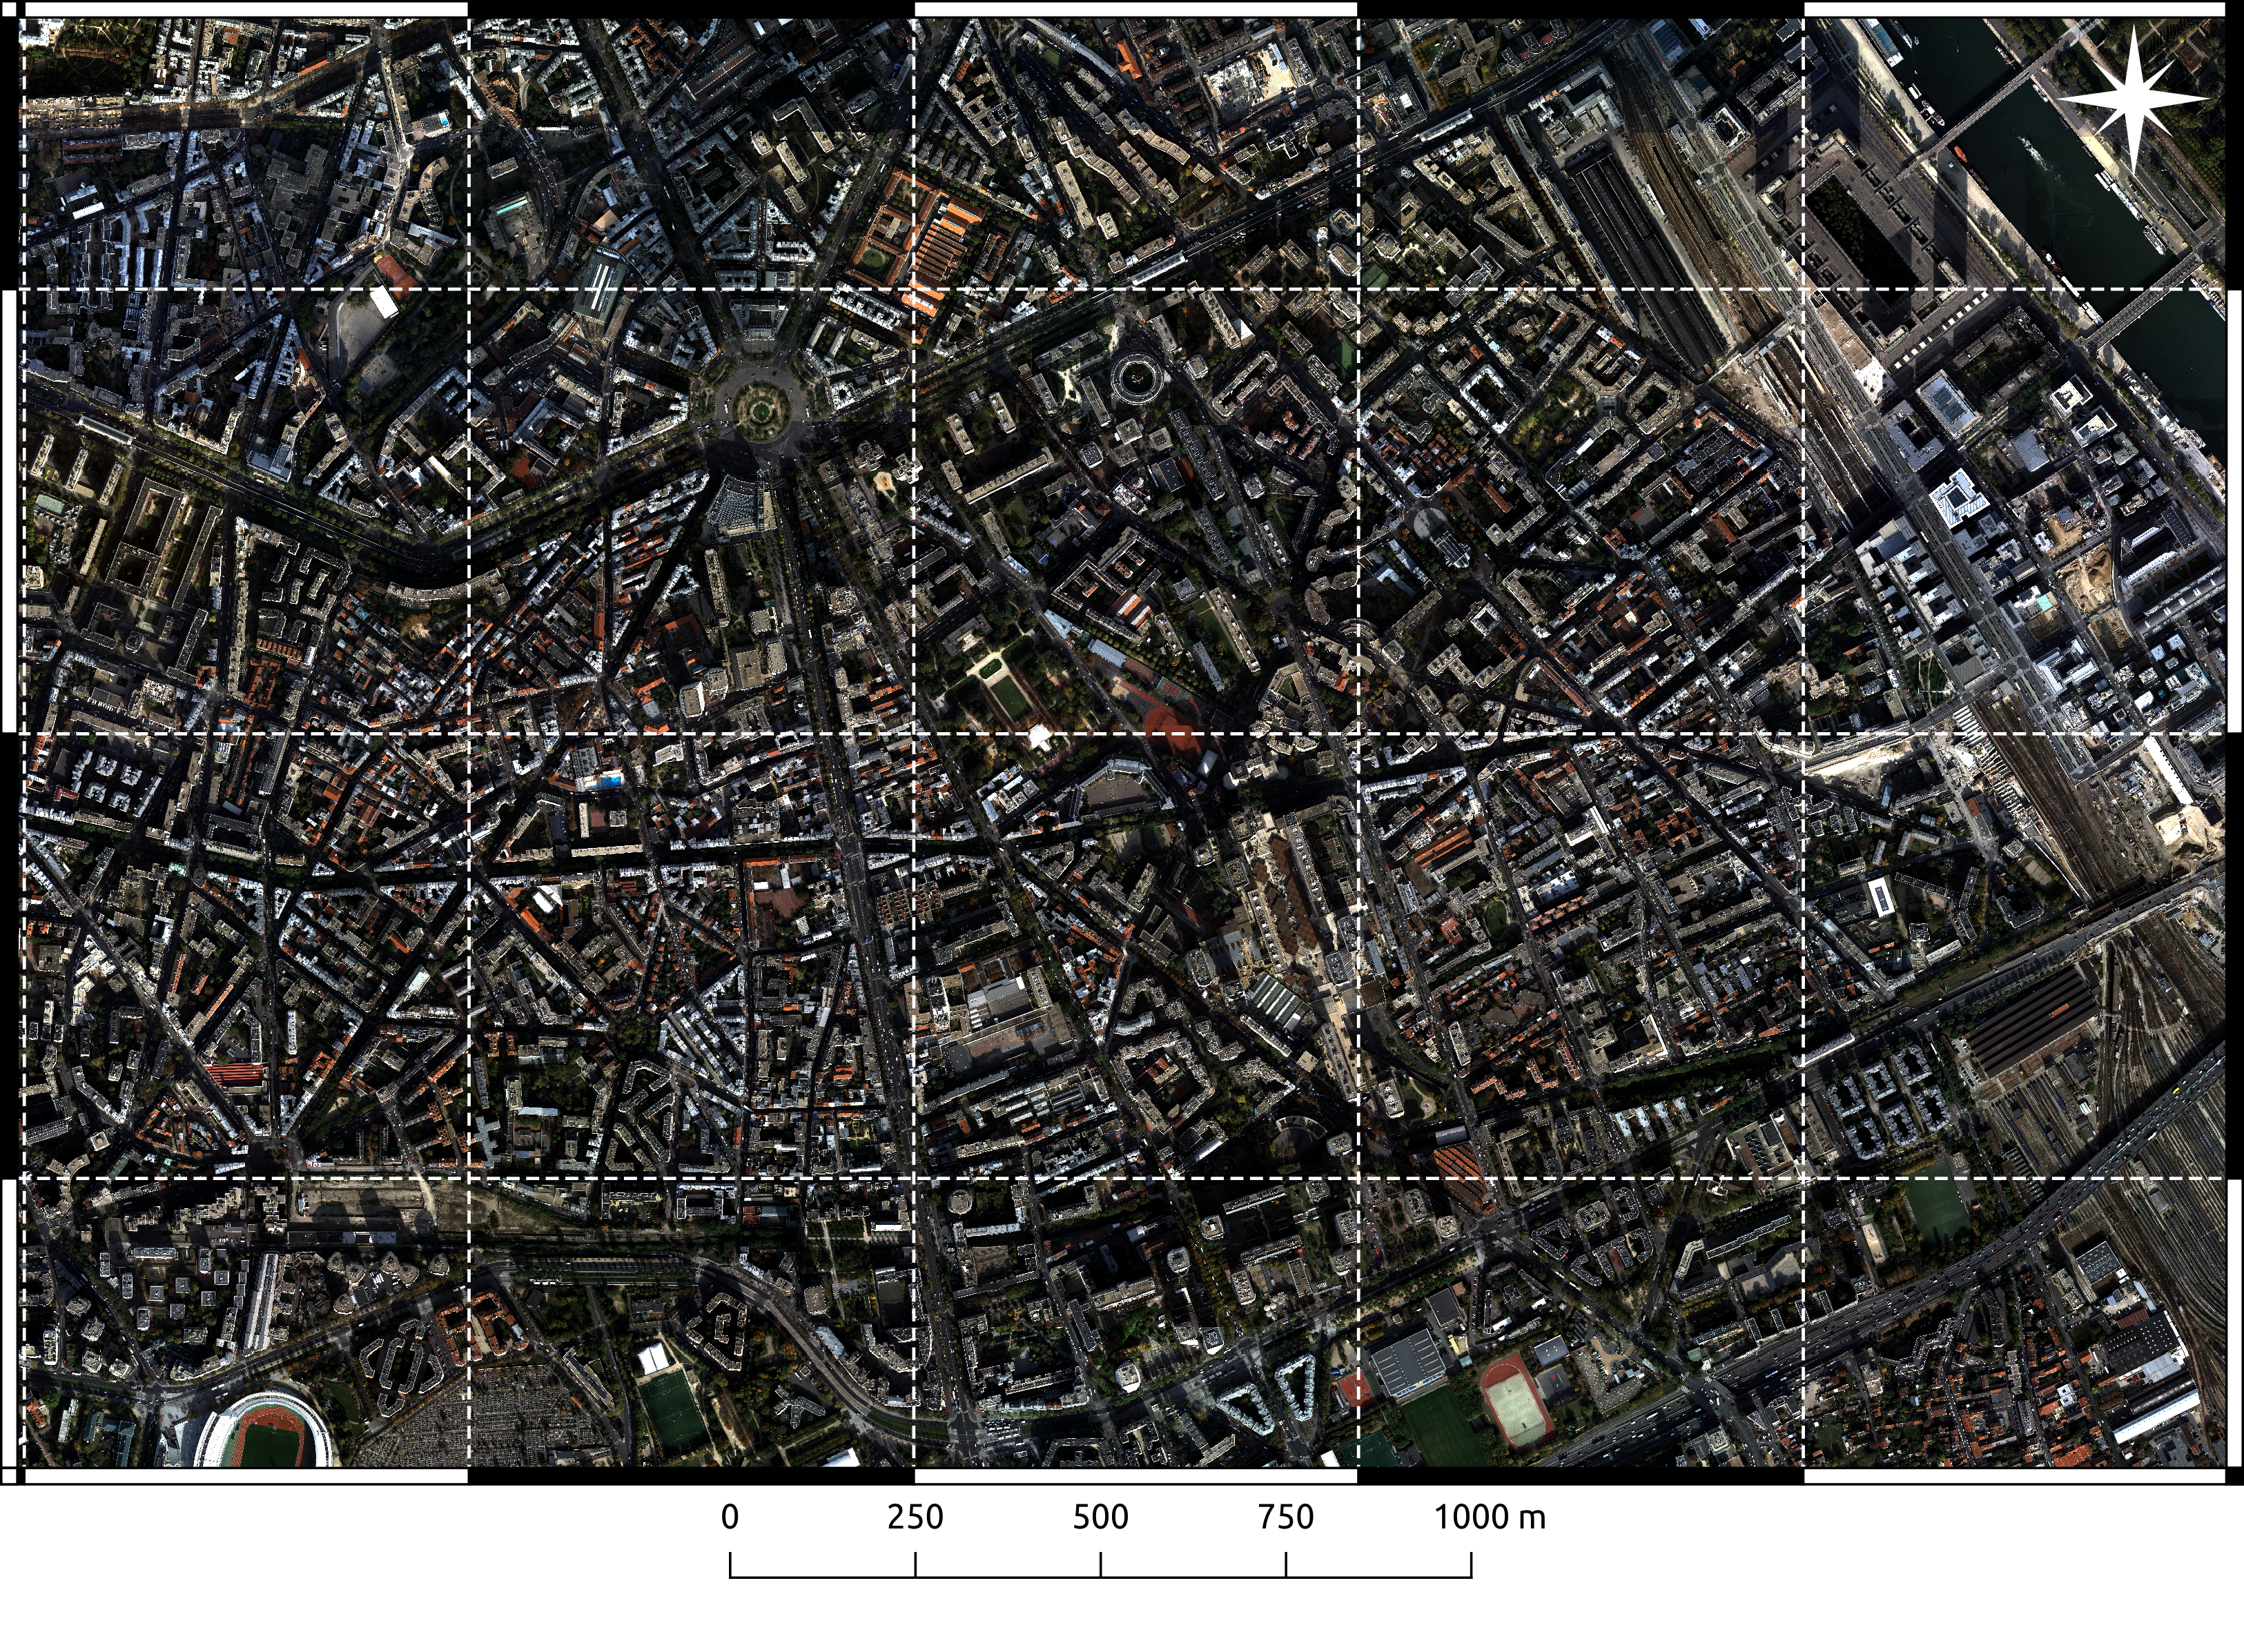
\includegraphics[width=\textwidth]{images/datasets/paris-13_global}
            }{
                \label{fig::paris-13_ortho}
                \caption{
                    Orthoimage showing the heterogeneous of the XIII\textsuperscript{th} district of Paris.
                }
            }
        \end{figure}

        \begin{figure}[htpb]
            \ffigbox[\textwidth]{
                \begin{subfloatrow}[3]
                    \ffigbox[\FBwidth]{
                        \includegraphics[width=.3\textwidth]{images/datasets/elancourt_samples}
                    }{
                        \label{subfig::elancourt_samples}
                        \caption{
                            Elancourt contains flat roof buildings (top) as well as gable roof ones (bottom).
                        }
                    }
                    \ffigbox[\FBwidth]{
                        \includegraphics[width=.3\textwidth]{images/datasets/nantes_samples}
                    }{
                        \label{subfig::nantes_samples}
                        \caption{
                            Nantes exhibits high rising towers (top) along side densely packed fragmented roof buildings (bottom).
                        }
                    }
                    \ffigbox[\FBwidth]{
                        \includegraphics[width=.3\textwidth]{images/datasets/paris-13_samples}
                    }{
                        \label{subfig::paris-13_samples}
                        \caption{
                            The XIII\textsuperscript{th} district of Paris is made of Haussmannian buildings (top) and high rising towers bottom).
                        }
                    }
                \end{subfloatrow}
            }{
                \label{fig::france_map}
                \caption{
                    Samples of building types per region.
                }
            }
        \end{figure}

        \gls{acr::3d} models were generated using the algorithm described in~\parencite{durupt2006automatic}, out of existing building footprints and aerial VHR multi-view \glspl{acr::dsm}.
        The modeling algorithm simulates possible roof structures with facets satisfying some geometric constraints.
        The best configuration is selected using a scoring system on the extrapolated roofs.
        Finally, vertical building fa\c{c}ades connect the optimal roof to the building footprint.
        These models have a \gls{acr::lod}-2 level.
        This method is adapted to roof types of low complexity and favors symmetrical models that are common in residential areas.
        It has been selected to ensure a varying error rate for the three areas of interest, especially since models were generated with partly erroneous cadastral maps.
        3,235 buildings in total are considered.
        They were annotated according to the atomic errors list provided by our taxonomy.

    \subsection{\textsc{Error statistics}}
        \label{subsec::experiments::datasets::stats}

        Some of the models obtained using the previous datasets were annotated manually in order to build training datasets.
        To annotate a building model, the manual operator compares the nadir projection of the model to the corresponding orthoimage and \gls{acr::dsm}.
        This was possible thanks to the work\footnote{\href{https://github.com/CHUPClem/sGrISner.git}{GIS Graphical interface for annotation.}} of Clémence Chupin, who was a Master student at \gls{acr::ensg}.
        Figure~\ref{fig::error_statistics} reports modeling errors statistics over the annotated buildings.

        \begin{figure}[htpb]
            \centering
            \ffigbox[\textwidth]{
                \includestandalone[mode=buildnew, width=\textwidth]{figures/datasets/families_stats}
            }{
                \caption{
                    \label{fig::family_errors}
                    Occurence statistics for error families computed for each area: \texttt{finesse} = 2.
                }
            }
        \end{figure}
        \begin{figure}[htpb]
            \centering
            \ffigbox[\textwidth]{
                \begin{subfloatrow}
                    \centering
                    \ffigbox[\textwidth]{
                        \includestandalone[mode=buildnew, width=\textwidth]{figures/datasets/lod1_stats}
                    }{
                        \caption{
                            \label{subfig::lod1_errors}
                            Occurence statistics for Building errors depending each area.
                        }
                    }
                \end{subfloatrow}
                \vskip1em
                \begin{subfloatrow}
                    \centering
                    \ffigbox[\textwidth]{
                        \includestandalone[mode=buildnew, width=\textwidth]{figures/datasets/lod2_stats}
                    }{
                        \caption{
                            \label{subfig::lod2_errors}
                            Occurence statistics for Facet errors depending each area.
                        }
                    }
                \end{subfloatrow}
            }{
                \label{fig::error_statistics}
                \caption{
                    Error statistics depending on the \texttt{finesse} level.
                    The height of bars indicates the frequency of each errors while the number of occurences is displayed over.
                }
            }
        \end{figure}

        These statistics are first analysed depending on the family errors at the \texttt{finesse} = 2 level (\textit{cf.} Figure~\ref{fig::family_errors}).
        Due to the fact that geometrically inconsistent \gls{acr::3d} models were filtered out in a preprocessing (nadir projection) step, \texttt{Unqualifiable} buildings represent a small fraction of the dataset (less than \SI{7.5}{\percent}).
        Actually, this latter corresponds to the, partially or completly, occluded buildings that could not be qualified.
        Moreover, only a small fraction of buildings are \texttt{Valid}:
        57 (\SI{2.84}{\percent}) in \textbf{Elancourt}, 55 (\SI{7.35}{\percent}) for \textbf{Nantes} and 21 (\SI{4.39}{\percent}) in \textbf{Paris-13}.
        Most buildings are affected by the \texttt{Building Errors} family (over \SI{58.16}{\percent}) and the \texttt{Facet Errors} one (over \SI{75.94}{\percent}).\\

        At the \texttt{finesse} level 3, two axes of analysis are possible.
        First, we group errors that are very frequent in the dataset.
        Over-segmentation errors (\texttt{FOS} and \texttt{BOS}), in both error families, are well represented ranging from \SIrange{38.9}{66.8}{\percent}.
        The same is true for \texttt{FIG} with a frequency from \SIrange{59.8}{80}{\percent}.
        \texttt{FIT}, on the other hand, are very rare in all the areas with ratios a little less than \SI{1.5}{\percent}.
        The rest have a presence ratio within the percentage interval of [10, 30].
        The errors that are rare are understandably going to impact negatively the learning process.\\
        
        Second, we can compare error frequency discrepancies depending on the studied scene.
        \textbf{Elancourt} is different compared to the relatively close sets \textbf{Nantes} and \textbf{Paris-13}, with regards to \texttt{BOS}, \texttt{BUS} and \texttt{BIT}.
        In fact, the last two areas are more densely urbanized than the first one exhibitting the same properties at \gls{acr::lod}-0.
        \texttt{BIB}, on the other hand, are equally distributed over the different datasets as it depends mostly on the input sensor data resolution independently of building types.\\
        At the facet level, \texttt{FIT} is also equally occuring across all the scenes different from the rest of \texttt{Facet errors}.
        In fact, \texttt{FOS} occurence ratio is related to the size of facets in urban scenes.
        Actually, the less complex roof structures are, the more big are facets and the more chance they have to be over segmented.
        Indeed, \textbf{Elancourt}, \textbf{Nantes} and \textbf{Paris-13} scenes are ordered in an ascending manner of their roof structure complexity.
        Conversely, in line with the previous analysis, \texttt{FUS} are less present in \textbf{Elancourt} than in \textbf{Nantes} which, in turn, contains less of the same error than \textbf{Paris-13}.
        \texttt{FIB} is distributed in the same manner as \texttt{FUS}.
        This is mainly due to the fact that the more a roof structure is complex the more precision errors are possible.
        \texttt{FIG} does not keep the same dynamic as its frequency keeps stable from \textbf{Elancourt} and \textbf{Nantes} but jumps considerably in \textbf{Paris-13}.
        This may be explained by the fact that the gap in \texttt{FUS} error ratios between \textbf{Paris-13} and \textbf{Nantes} is more important than that of \texttt{FOS} errors, contrarily to the same gaps for the same errors between \textbf{Nantes} and \textbf{Elancourt} which compensate each other.

\section{\textsc{Pipeline evaluation}}
    \label{sec::experiments::evaluation}
    In the last section, we also explained how we acquired our dataset, in addition to analysing the effect of the urban scene on error statistics.
    Beforehand, all the ingredients needed in the proposed methodology were presented.
    This section aims at specifying how each bloc of the pipeline is implemented.\\

    In Subsection~\ref{subsec::experiments::evaluation::setup} provides all details about our experimental approach.
    Next in Subsection~\ref{subsec::experiments::evaluation::baseline_feature_analysis}, we report some first results using the baseline features we developped.

    \subsection{\textsc{Experimental set-up}}
        \label{subsec::experiments::evaluation::setup}
        In this subsection, we give detailed account of how every building block of our pipeline is parameterized.
        We first start by discussing feature configurations, before defining the taxonomy parameters of interest and endin with a thorough description of the classification process.

        \subsubsection{\textsc{Feature configurations}}
            \label{subsubsec::experiments::evaluation::setup::feature_configurations}
            We present herein the features that were used in experiments.
            First, as we tried to prove the efficiency of the proposed learning framework, we made use different configurations using the baseline features.
            Second, as richer features were used, new combinations were possible and are discussed hereafter.

            \paragraph{Baseline features}
                The geometric features are always available.
                As a consequence, we tested four feature configurations: ``geometric features'' (\textbf{Geom.}) only, ``geometric and height features''(\textbf{Geom.} $\cup$ \textbf{Hei.}), ``geometric and image features''(\textbf{Geom.} $\cup$ \textbf{Im.}) as well as ``geometric, height and image features''(\textbf{All.}).
                In order to have a better compare the important of each modality, the feature vectors they produce are of the same size.
                Actually, using the function \(\chi_{\max,\min,\operatorname{mean},\operatorname{med}}\) defined in Equation~\ref{eq::max_min_mean_med_extractor}, the geometric feature vector in Equation~\ref{eq::geometric_features} is of dimension
                \begin{equation*}
                    \underbrace{4}_{\substack{\text{the output dimension}\\\text{of the function } \chi_{\max,\min,\operatorname{mean},\operatorname{med}} }} \times \underbrace{5}_{\substack{\text{the number of the facet}\\\text{graph attributes}}} = 20.
                \end{equation*}

                Regarding height based feature vectors their dimension depend on the histogram parameters.
                Since we compute differences between observed and model height at terrain level also (\textit{cf.} Subsection~\ref{subsec::learned_evaluation::baseline::height}), and because these are virtually unbounded and can differ from one scene to another, the maximum possible discrepancy is limited to \SI{\pm 50}{\m} for all scenes.
                In order to have the same feature vector dimension for this modality, the number of bins is fixed manually to \(20\).
                For image based features, the cosine similarity between normal vectors, used in Equation~\ref{eq::corr_fac}, is by definition bounded in the interval [-1, 1].
                This interval is consequently divided evenly into \(20\) bins for the histogram computation.
                The \glspl{acr::dsm} and orthorectified images used to derive height and image features have the same spatial resolution as the reconstruction input data.\\

                time= ??

            \paragraph{Richer features}
                Baseline features are replaced by more enhanced ones as shown in Section~\ref{sec::learned_evaluation::richer_features}.
                We lay out herein how their parameters are determined.

                \subparagraph{Graph kernels}
                    In Subsection~\ref{subsec::learned_evaluation::richer_features::graph}, we have seen how 14 graph kernels are aggregated to describe graphs.
                    We provide herein the parameters of each kernel type.
                    \begin{description}
                        \item[Random walk] The exponential version did not seem to converge and was left out.
                                    After a grid search \(\lambda\) was set to be \num{1e-3}, for the geometric random walk.
                        \item[\gls{acr::svm} \(\vartheta\)] This kernel takes no parameters.
                        \item[] 
                    \end{description}

                \subparagraph{\gls*{acr::scatnet}}
                    
                scatnet J 3 L 8 kymatio
                % # features = ?
                random walk grakel
                graph hopper
                propagation
                multilaplacian= ?

                times


        \subsubsection{\textsc{Considered labels}}
            All \textbf{\gls{acr::efin}} levels were tested.
            The input models are generalized to \gls{acr::lod}-2.
            As a consequence, we chose \textbf{\gls{acr::elod}} = \gls{acr::lod}-2.
            If the \textbf{exclusivity} is \textsc{on}, at \textbf{\gls{acr::efin}} level 3, the second stage classification results depends on the first one.
            We are, at this stage, trying to prove the feasability, in the first place, of the proposed approach.
            As proven in the latter experiments (\textit{cf.} Section~\ref{sec::more_experiments::finesse}), the first stage results are not good enough in order to test this configuration.
            That is why we limited the experiments to the case where the \textbf{exclusivity} is set to be \textsc{off}.

        \subsubsection{\textsc{Classification settings}}
            Herein, are given extensive details how the considered classifiers (\textit{cf.} Subsection~\ref{subsec::learned_evaluation::classification::classifiers}) are applied.
            We also provide the metrics that will help measure the accuracy of predictions.

            \paragraph{Classifiers}
                As discussed in Subsection~\ref{subsec::learned_evaluation::classification::classifiers}, two classifier types were considered in the experimental study.
                As already explained beforehand in Subsection~\ref{subsec::learned_evaluation::classification::classifiers}, a one-vs-all approach is used to adapt \glspl{acr::rf} to multi-label settings.
                The same approach was choosen to accommodate \glspl{acr::svm} to both the multi-class and the multi-label possibilities.
                We relied upon the already available and ubequitous implementation in Python~\parencite{scikit-learn}.
                Below we detail quantitavely the used parameters.
                
                \sisetup{
                    scientific-notation = true
                }
                \subparagraph{\acrshort*{acr::rf}}
                    A brief grid search involving a smaller set of building models and only baseline geometric features~\parencite{ennafii2018qualificationunannotated} yielded comparable results for the number of trees set in the range \numrange{850}{1000} and a maximum tree depth from \numrange{3}{5}.
                    Given the already immense parameter search space involving all possible feature configurations, feature extraction parameters and label possibilities, the \gls{acr::rf} parameters are set to \num{1000} for the tree number and 4 for the maximum tree depth for all other experiments without performing any grid search.
                    Regarding \gls{acr::scatnet} based features, in Subsection~\ref{subsec::more_experiments::richer_features::scatnet_baseline} were reduced using \gls{acr::pca} and Kernel\footnote{The used kernel is that same the one used with the \gls{acr::svm} classifier.} \gls{acr::pca} in order to not overwhelm the geometric features.
                    To that end, these rich features are reduced to 20 in length to equal the dimension of baseline geometric feature vectors.

                \subparagraph{\acrshort*{acr::svm}}
                    The linear \gls{acr::svm} is not well suited for the type of features that we use, even for baseline features as experiments do not yield any resuslts in time.
                    As a consequence, the latter was left out and we experimented only with the kernel \gls{acr::svm} using the standard \gls{acr::rbf} kernel (\textit{cf.} Equation~\ref{eq::rbf_kernel}) when instances are vectors not graphs.
                    Just as with the \gls{acr::rf} classifier, we conducted a grid search using baseline geometric features only in order to determine both parameters \(C\) and \(\gamma\) by limiting the range between \numrange[range-phrase={ and }]{1e1}{1e-3} for both.
                    All values yielded sensibly the same scores.
                    As a result we set these parameters as follows: \(C = \num{1e-1}\) to not overpenalize nor underfit during learning and \(\gamma = \num{1e-3}\) to avoid overfitting.
                    Regarding \gls{acr::mkl}, we made use of the already implemented EasyMKL~\parencite{aiolli2015easymkl} approach.
                    It was the only method, to our knowledge that was readily available library to use with Python\footnote{\href{https://github.com/IvanoLauriola/MKLpy}{MKLpy}}.
                    \sisetup{
                        scientific-notation = false
                    }
    
            \paragraph{Used metrics}
                The overall accuracy is not interesting due to the highly unbalanced label distribution.
                We prefer reporting recall \(\bm{Rec}\) and precision \(\bm{Prec}\) ratios.
                As a reminder these metrics are defined as follows:
                \begin{align}
                    \label{eq::recall_precision}
                    \bm{Rec} &\triangleq \frac{tp}{tp + fp}\\
                    \bm{Prec} &\triangleq \frac{tp}{tp + fn},
                \end{align}
                where:
                \begin{conditions}
                    tp & the number of instances predicted positive that are positive in reality;\\
                    fp & the number of instances predicted positive that are negative in reality;\\
                    fn & the number of instances predicted negative that are positive in reality.
                \end{conditions}
                Recall expresses, from a number of samples of a given class, the proportion that was rightfully detected as such.
                Precision indicates how much samples, amongst the detected ones, were, in truth, part of the studied class~\parencite{powers2011evaluation}.
                We also summarize these two ratios with their harmonic mean, the F-score:
                \begin{equation}
                    \label{eq::f_score}
                    \bm{F_{score}} \triangleq \frac{2}{\frac{1}{\bm{Rec}} + \frac{1}{\bm{Prec}}}.
                \end{equation}
                Unless said otherwise, all experiments were conducted performing a 10-fold cross validation to avoid overfitting or underfitting issues.
                Only test results are reported.

    \subsection{\textsc{Baseline feature analysis}}
        \label{subsec::experiments::evaluation::baseline_feature_analysis}
        At this stage, we study only the baseline features proposed in Section~\ref{sec::learned_evaluation::baseline}.
        The goal is to assess the added value of each modality.
        First, the \gls{acr::rmse} is proven to be inadequate for detecting errors in our taxonomy.
        Second, prediction results from all possible feature configurations are compared in Subsubsection~\ref{subsubsec::experiments::evaluation::setup::feature_configurations}.
        Third and last, we conclude the analysis by studying the feature importance, for all training zones.

        \subsubsection{\textsc{\acrshort*{acr::rmse} predictive capacity}}
            \label{subsubsec::experiments::evaluation::baseline_feature_analysis::rmse}
            The \gls{acr::rmse} is the standard measure in most of \gls{acr::3d} reconstruction methods.
            As a consequence, we use it herein as a reference that our baseline is to be compared to.
            We train the classifier on Elancourt with the one dimensional feature vector containing the \gls{acr::rmse}.
            This scene was sufficient enough for our analysis.
            Mean test results are shown in Table~\ref{tab::rmse_results}.\\

            \begin{table}[htpb]
                \begin{tabular}{c c c c c c c c c c}
                    \toprule
                    & \texttt{BOS} & \texttt{BUS} & \texttt{BIB} & \texttt{BIT} & \texttt{FOS} & \texttt{FUS} & \texttt{FIB} & \texttt{FIT} & \texttt{FIG} \\
                    \midrule
                    \(\bm{Rec}\) & 99.55 & 0.21 & 0 & 0 & 98.68 & 0.63 & 0 & 0 & 98.15 \\
                    \midrule
                    \(\bm{Prec}\) & 68.78 & 33.33 & --- & 0 & 66.60 & 0.25 & --- & 0 & 61.15 \\
                    \midrule
                    \(\bm{F_{score}}\) & 81.35 & 0.42 & 0 & 0 & 79.52 & 1.24 & 0 & 0 & 75.36 \\
                    \midrule
                    \(\bm{Acc}\) & 68.46 & 75.65 & 89.57 & 94.66 & 66.36 & 83.62 & 88.24 & 98.36 & 60.86 \\
                    \bottomrule
                \end{tabular}
                \caption{
                    \label{tab::rmse_results} \texttt{Finesse} 3 experiment results using \gls{acr::rmse} on Elancourt.
                    \(\bm{Acc}\) expresses the overall accuracy ratio.
                }
            \end{table}

            We can distinguish two groups of errors: 
            \begin{description}
                \item[\texttt{BOS}, \texttt{FOS} and \texttt{FIG}:] These have a high recall and a low precision and overall accuracy;
                \item[\texttt{BUS}, \texttt{BIB}, \texttt{BIT}, \texttt{FUS}, \texttt{FIB} and \texttt{FIT}:] These have low recall and precision ratios.
            \end{description}
            The first (\textit{resp.} second) group coincides exactly with errors that affect more (\textit{resp.} less) than half of the buildings.
            For this kind of errors, the classifier assigns to almost all samples the positive class.
            In fact, we end up with a high ratio of false positives (false alarms) and hence a high recall ratio that is coupled with a weak precision and overall accuracy.
            Exactly the inverse happens with the rest of the errors as we obtain a high percentage of false negative.
            We can safely conclude that the \gls{acr::rmse} is not able to detect errors defined in our taxonomy.

        \subsubsection{\textsc{Feature ablation study}}
            \label{subsubsec::experiments::evaluation::baseline_feature_analysis::ablation}
            We tested the different feature configurations, at \texttt{finesse} level 3 and in all urban zones.
            Mean precision and recall test results are reported in Table~\ref{tab::ablation_f3}.
            F-scores are averaged across all feature configurations and represented in Figure~\ref{fig::f_score_ablation_f3}.\\

            \begin{table}[htpb]
                \small
                \begin{center}
                    \begin{tabular}{| c | c c | c c | c c | c c |}
                        \hline
                        \multicolumn{9}{|c|}{\textbf{Elancourt}}\\
                        \hline
                        &\multicolumn{2}{c|}{\textbf{Geom.}} & \multicolumn{2}{c|}{\textbf{Geom. $\cup$ Hei.}} & \multicolumn{2}{c|}{\textbf{Geom. $\cup$ Im.}} & \multicolumn{2}{x{2.4cm}|}{\textbf{All}}\\
                        \cline{2-9}
                        & \(\bm{Rec}\) & \(\bm{Prec}\) &  \(\bm{Rec}\) & \(\bm{Prec}\) &  \(\bm{Rec}\) & \(\bm{Prec}\) &  \(\bm{Rec}\) & \(\bm{Prec}\) \\
                        \hline
                        \texttt{BOS} & \textbf{93.96} & 76.15 & 91.43 & \textbf{77.76} & 91.51 & 76.08 & 90.83 & 76.14 \\
                        \hline
                        \texttt{BUS} & 32.98 & \textbf{76.47} & \textbf{41.86} & 75.57 & 40.38 & 71.00 & 39.32 & 71.81 \\
                        \hline
                        \texttt{BIB} & 12.32 & 67.57 & 12.81 & \textbf{68.42} & 16.26 & 67.35 & \textbf{16.75} & 68.0 \\
                        \hline
                        \texttt{BIT} & \textbf{25.25} & 92.59 & 20.20 & 90.91 & 20.20 & \textbf{95.24} & 11.11 & 91.67 \\
                        \specialrule{.2em}{.1em}{.1em}
                        \texttt{FOS} & 98.91 & 99.07 & 98.91 & \textbf{99.30} & \textbf{98.99} & 98.84 & 98.91 & 98.84 \\
                        \hline
                        \texttt{FUS} & \textbf{1.90} & 54.55 & 0.63 & \textbf{66.67} & 1.61 & 50 & 1.27 & \textbf{66.67} \\
                        \hline
                        \texttt{FIB} & \textbf{9.17} & 87.5 & 0 & --- & 8.30 & 82.61 & 7.42 & \textbf{100} \\
                        \hline
                        \texttt{FIT} & 6.67 & \textbf{100} & \textbf{8.73} & 95.24 & 3.33 & \textbf{100} & 3.33 & \textbf{100} \\
                        \hline
                        \texttt{FIG} & \textbf{80.54} & 73.14 & 80.45 & \textbf{72.62} & 78.69 & 72.12 & 79.02 & 71.82 \\
                        \hline
                        \hline
                        \multicolumn{9}{|c|}{\textbf{Nantes}}\\
                        \hline
                        &\multicolumn{2}{c|}{\textbf{Geom.}} & \multicolumn{2}{c|}{\textbf{Geom. $\cup$ Hei.}} & \multicolumn{2}{c|}{\textbf{Geom. $\cup$ Im.}} & \multicolumn{2}{x{2.4cm}|}{\textbf{All}}\\
                        \cline{2-9}
                        & \(\bm{Rec}\) & \(\bm{Prec}\) &  \(\bm{Rec}\) & \(\bm{Prec}\) &  \(\bm{Rec}\) & \(\bm{Prec}\) &  \(\bm{Rec}\) & \(\bm{Prec}\) \\
                        \hline
                        \texttt{BOS} & \textbf{38.14} & 61.67 & 36.43 & 60.23 & 36.77 & \textbf{62.21} & 34.71 & 60.48 \\
                        \hline
                        \texttt{BUS} & 7.35 & 62.5 & 7.35 & 55.56 & \textbf{29.41} & \textbf{66.67} & 26.47 & 64.29 \\
                        \hline
                        \texttt{BIB} & 0 & --- & 0 & --- & \textbf{1.01} & \textbf{50.0} & \textbf{1.01} & \textbf{50.0} \\
                        \hline
                        \texttt{BIT} & 1.77 & 22.22 & \textbf{3.54} & 44.44 & 0 & 0 & 2.65 & \textbf{50.0} \\
                        \specialrule{.2em}{.1em}{.1em}
                        \texttt{FOS} & \textbf{98.54} & \textbf{98.13} & \textbf{98.54} & \textbf{98.13} & 98.33 & 97.92 & 98.12 & 97.91 \\
                        \hline
                        \texttt{FUS} & 27.62 & 55.24 & \textbf{27.62} & \textbf{59.18} & 24.76 & 54.74 & 23.33 & 53.85 \\
                        \hline
                        \texttt{FIB} & 37.80 & 62.0 & 36.59 & \textbf{63.16} & \textbf{49.39} & 60.90 & 46.39 & 60.90 \\
                        \hline
                        \texttt{FIT} & 0 & --- & 0 & --- & 0 & --- & 0 & --- \\
                        \hline
                        \texttt{FIG} & 86.32 & 78.09 & \textbf{86.77} & 78.02 & 84.53 & \textbf{78.71} & 83.86 & 78.08 \\
                        \hline
                        \hline
                        \multicolumn{9}{|c|}{\textbf{Paris-13}}\\
                        \hline
                        &\multicolumn{2}{c|}{\textbf{Geom.}} & \multicolumn{2}{c|}{\textbf{Geom. $\cup$ Hei.}} & \multicolumn{2}{c|}{\textbf{Geom. $\cup$ Im.}} & \multicolumn{2}{x{2.4cm}|}{\textbf{All}}\\
                        \cline{2-9}
                        & \(\bm{Rec}\) & \(\bm{Prec}\) &  \(\bm{Rec}\) & \(\bm{Prec}\) &  \(\bm{Rec}\) & \(\bm{Prec}\) &  \(\bm{Rec}\) & \(\bm{Prec}\) \\
                        \hline
                        \texttt{BOS} & 45.54 & 65.25 & 46.53 & 68.61 & \textbf{50.0} & 68.24 & 46.53 & \textbf{70.15} \\
                        \hline
                        \texttt{BUS} & 6.35 & 66.67 & 7.94 & 71.43 & \textbf{22.22} & \textbf{77.78} & 7.94 & 62.5 \\
                        \hline
                        \texttt{BIB} & 0 & --- & 0 & --- & 0 & 0 & 0 & --- \\
                        \hline
                        \texttt{BIT} & \textbf{2.63} & \textbf{50.0} & 0 & --- & 1.32 & 50.0 & 0 & 0 \\
                        \specialrule{.2em}{.1em}{.1em}
                        \texttt{FOS} & 97.19 & 97.19 & 97.19 & 97.19 & \textbf{97.59} & \textbf{98.38} & 97.19 & 97.19 \\
                        \hline
                        \texttt{FUS} & \textbf{85.09} & \textbf{75.0} & 84.36 & 74.12 & 85.09 & 74.52 & 84.36 & 74.12 \\
                        \hline
                        \texttt{FIB} & 53.47 & 62.10 & 51.39 & 61.67 & \textbf{53.47} & \textbf{63.11} & 52.78 & 61.79 \\
                        \hline
                        \texttt{FIT} & 0 & --- & 0 & --- & 0 & --- & 0 & --- \\
                        \hline
                        \texttt{FIG} & 97.65 & 84.62 & \textbf{98.96} & \textbf{84.79} & 97.65 & 84.62 & \textbf{98.96} & \textbf{84.79} \\
                        \hline
                    \end{tabular}
                \end{center}
                \caption{
                    \label{tab::ablation_f3} Feature ablation study preformed on the three areas at \texttt{finesse} level 3.
                    Test results are expressed in percentage.
                    All \texttt{atomic} errors are considered over all possible configurations.
                }
            \end{table}

            \thisfloatsetup{subfloatrowsep=none}
            \begin{figure}[htpb]
                \centering
                \ffigbox[\FBwidth]{
                    \begin{subfloatrow}[2]
                        \ffigbox[\FBwidth]{
                            \includestandalone[mode=buildnew, height=7.5cm]{figures/results/ablation/building}
                        }{
                            \caption{
                                \label{subfig::f_score_ablation_f3_building}
                                \texttt{Building errors.}
                            }
                        }
                        \ffigbox[\FBwidth]{
                            \includestandalone[mode=buildnew, height=7.5cm]{figures/results/ablation/facet}
                        }{
                            \caption{
                                \label{subfig::f_score_ablation_f3_facet}
                                \texttt{Facet errors.}
                            }
                        }
                    \end{subfloatrow}
                }{
                    \caption{
                        \label{fig::f_score_ablation_f3}
                        Mean F-score and standard deviation for the feature ablation study.
                    }
                }
            \end{figure}

            First, we can point out that fact that geometric features alone are generally sufficient.
            It is actually the best alternative for topological error detection as shown for \texttt{BOS}, \texttt{FOS}, \texttt{FUS}, \texttt{FIT} and \texttt{BIT} in Table~\ref{tab::ablation_f3}.
            This is confirmed also by the low variance observed in Subfigure~\ref{subfig::f_score_f3_building}.
            An exception is noticed with \texttt{BUS} in \textbf{Elancourt}, where height-based features allow an increase of around \SI{9}{\percent} in recall without, practically, any loss in precision.
            Similar behaviour is noticed for \textbf{Nantes} and \textbf{Paris-13} with image-based features (+\SI{20}{\percent} in recall).
            The first case can be explained by the discrepancy in height that can be observed between under-segmented buildings.
            The second is made clear by the difference in roof colors, in dense uniform settings (Subfigure~\ref{subfig::bus_2d}).
            This helps identifying different instances of buildings.\\

            Figure~\ref{fig::f_score_ablation_f3} shows that all \texttt{Building errors} labels are better detected in \textbf{Elancourt}.
            It is also the case of \texttt{FOS} and \texttt{FIT}.
            A certain monotony can be noticed, at the exception of \texttt{BOS}.
            Better resultas are obtained for \textbf{Paris-13} than for \textbf{Nantes}, while having around half the number of models to train on.
            This means that \texttt{BOS} cannot be easily learnt in \textbf{Nantes}.
            It is coherent with the fact that the dataset represents a part of the dense downtown of the city.
            The same monotony is observed, this time in reverse, with the rest of \texttt{Facet errors} defects. \textbf{Paris-13} is much better with less training samples.
            For geometric defects (\texttt{FIG} and \texttt{FIB}), \textbf{Nantes} is comparable to \textbf{Paris-13}, but, with \texttt{FUS}, it is way much worse.
            This may result from the highly heterogeneous aspect of this dataset that encompasses high tower buildings with a densely populated city district.
            Finally, well represented errors are more easily detected than the less frequent ones, especially the rare ones like \texttt{FIT} in \textbf{Nantes} and \textbf{Paris-13}.
        
        \subsubsection{\textsc{Feature importance}}
            \label{subsubsec::experiments::evaluation::baseline_feature_analysis::feature_importance}
            \gls{acr::rf} classifiers can easily infer feature importances at training time.
            These were here computed and aggregated by modality in all urban scenes (\textit{cf.} Figure~\ref{fig::feature_importances}).\\

            \begin{figure}[htpb]
                \centering
                \ffigbox[\textwidth]{
                    \begin{subfloatrow}
                        \ffigbox[\textwidth]{
                            \includestandalone[mode=buildnew, width=.8\textwidth]{figures/results/feature_importance/building}
                        }{
                            \caption{
                                \label{subfig::feature_importances_building}
                                \texttt{Building errors.}
                            }
                        }
                    \end{subfloatrow}
                    \vskip1em
                    \begin{subfloatrow}
                        \ffigbox[\textwidth]{
                            \includestandalone[mode=buildnew, width=\textwidth]{figures/results/feature_importance/facet}
                        }{
                            \caption{
                                \label{subfig::feature_importances_facet}
                                \texttt{Facet errors.}
                            }
                        }
                    \end{subfloatrow}
                }{
                    \caption{
                        \label{fig::feature_importances} Modality importance computed by stacking single feature importances retrieved from the \gls{acr::rf} classifier.
                        The first (\textit{resp.} second and third) column represents \textbf{Elancourt} (\textit{resp.} \textbf{Nantes} and \textbf{Paris-13}).
                    }
                }
            \end{figure}
            
            At first, we observe how much individual attributes are important before being gathered.
            For geometric features, all attributes are equally important.
            However, concerning image and height-based features, only a few are relevant (higher feature importance ratio).
            Indeed, these few attributes correspond to the highest and lowest values of the histograms.
            As described earlier, image and height features consist of a histogram of distances between the model and the real measured signals:
            vector cosine similarity, for the first, and the \(L_2\) norm for the last.
            It is clear that the presence of errors would result in saturating the high values in the histogram, while an absence of defects would imply a big number of low values.
            This intuitively explains the observed phenomenon.
            
            In a second time, we notice that no modality is more important than the others, contrarily to what was observed in Table~\ref{tab::ablation_f3}.
            In fact, for most atomic errors, test results using geometric features are comparable to those obtained with more modalities.
            However, during training, all modalities are relevant ($\sim$1/3 in Figure~\ref{fig::feature_importances}).
            This explains why all configurations are kept for subsequent analysis.
